\chapter{Daq information}
\label{app:three}

This chapter summarizes the minimum information from the DAQ needed for the analysis.

\section{DAQ}

\subsection{Header information}
This section provides the information regarding user interface to the event, AMC13 and rider header information. All the information are stored in the art/ROOT files and standalone ROOT files with the TBranch structures in the following sections.

\subsection{Header and trailer formats}

This section compiles all the available header data formats. Please refer to \url{http://gm2-docdb.fnal.gov:8080/cgi-bin/ShowDocument?docid=3409} for more details.

\begin{figure}[htbp]
\centering
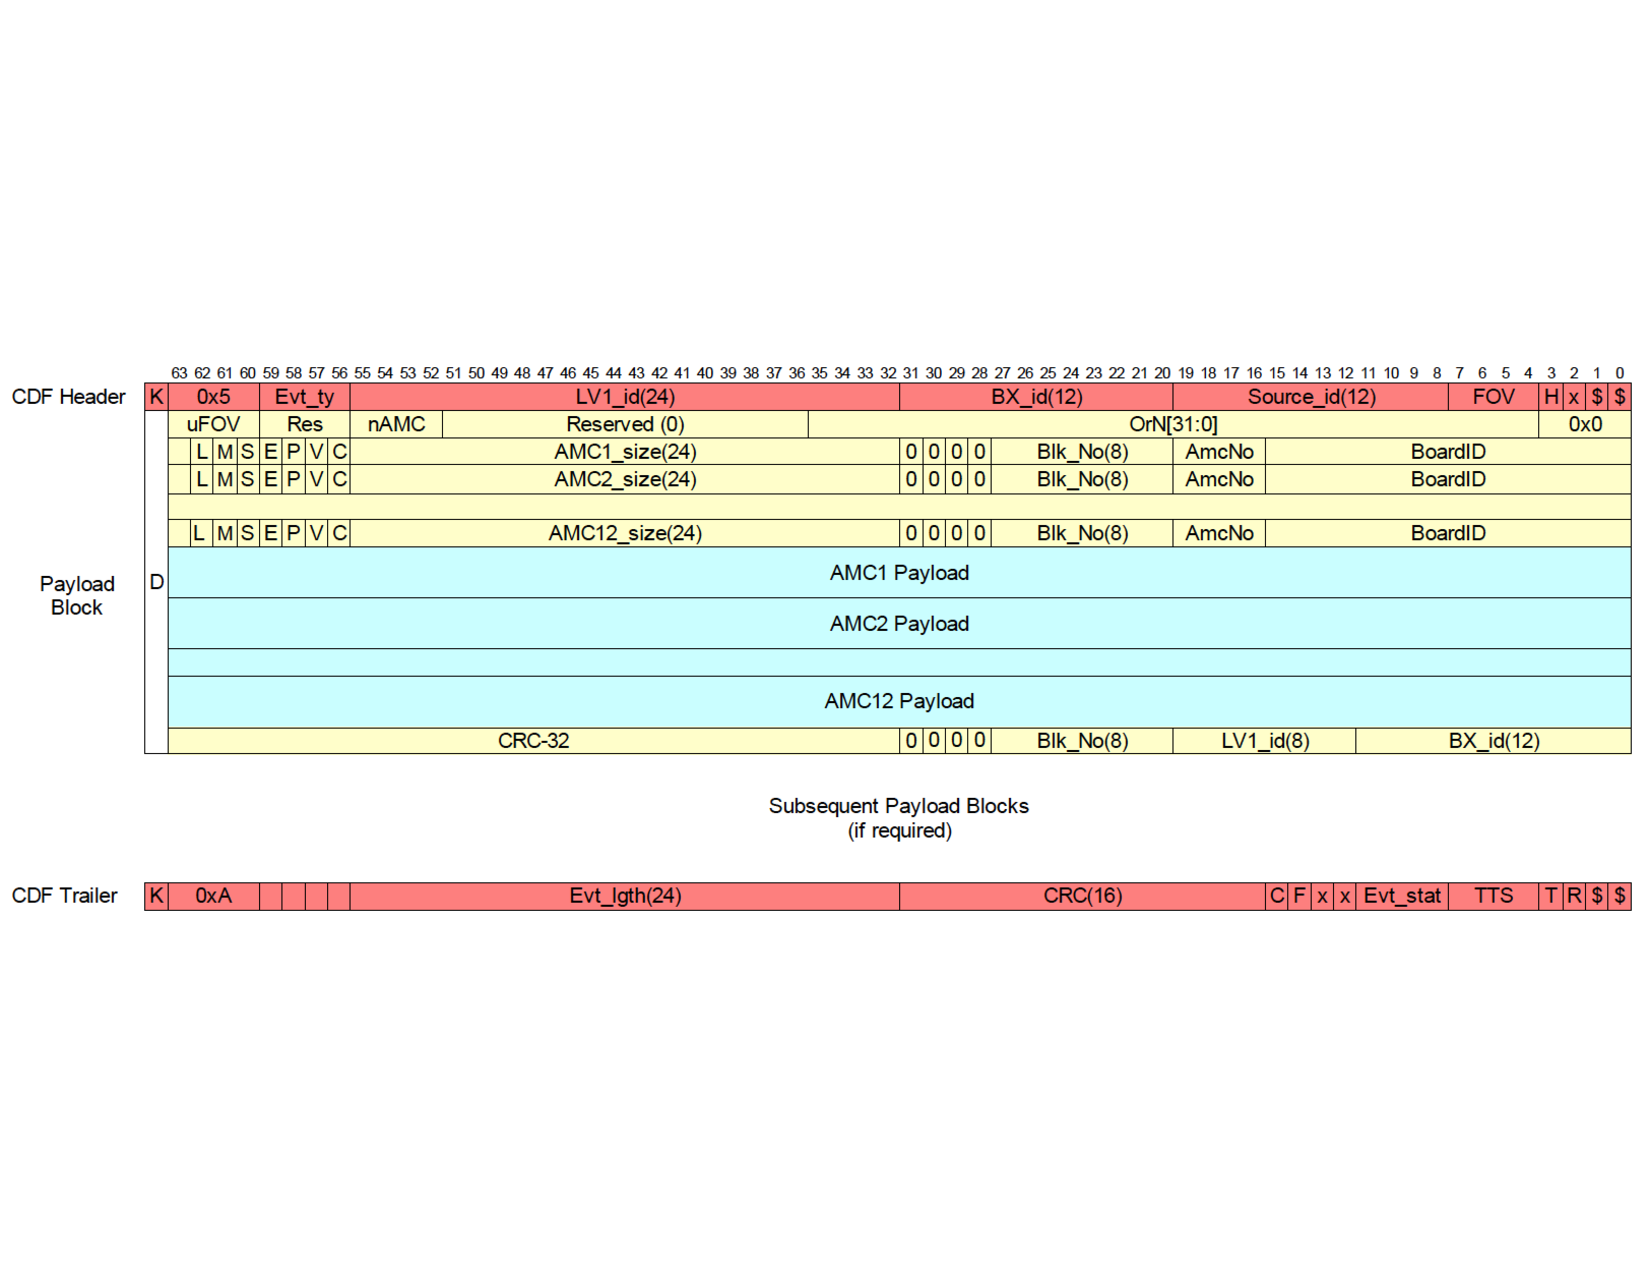
\includegraphics[trim=0cm 6cm 0cm 6cm ,width=0.95\textwidth]{pics/AMC13Header}
\caption{AMC13 to DAQ data format.}
\end{figure}

\begin{figure}[htbp]
\centering
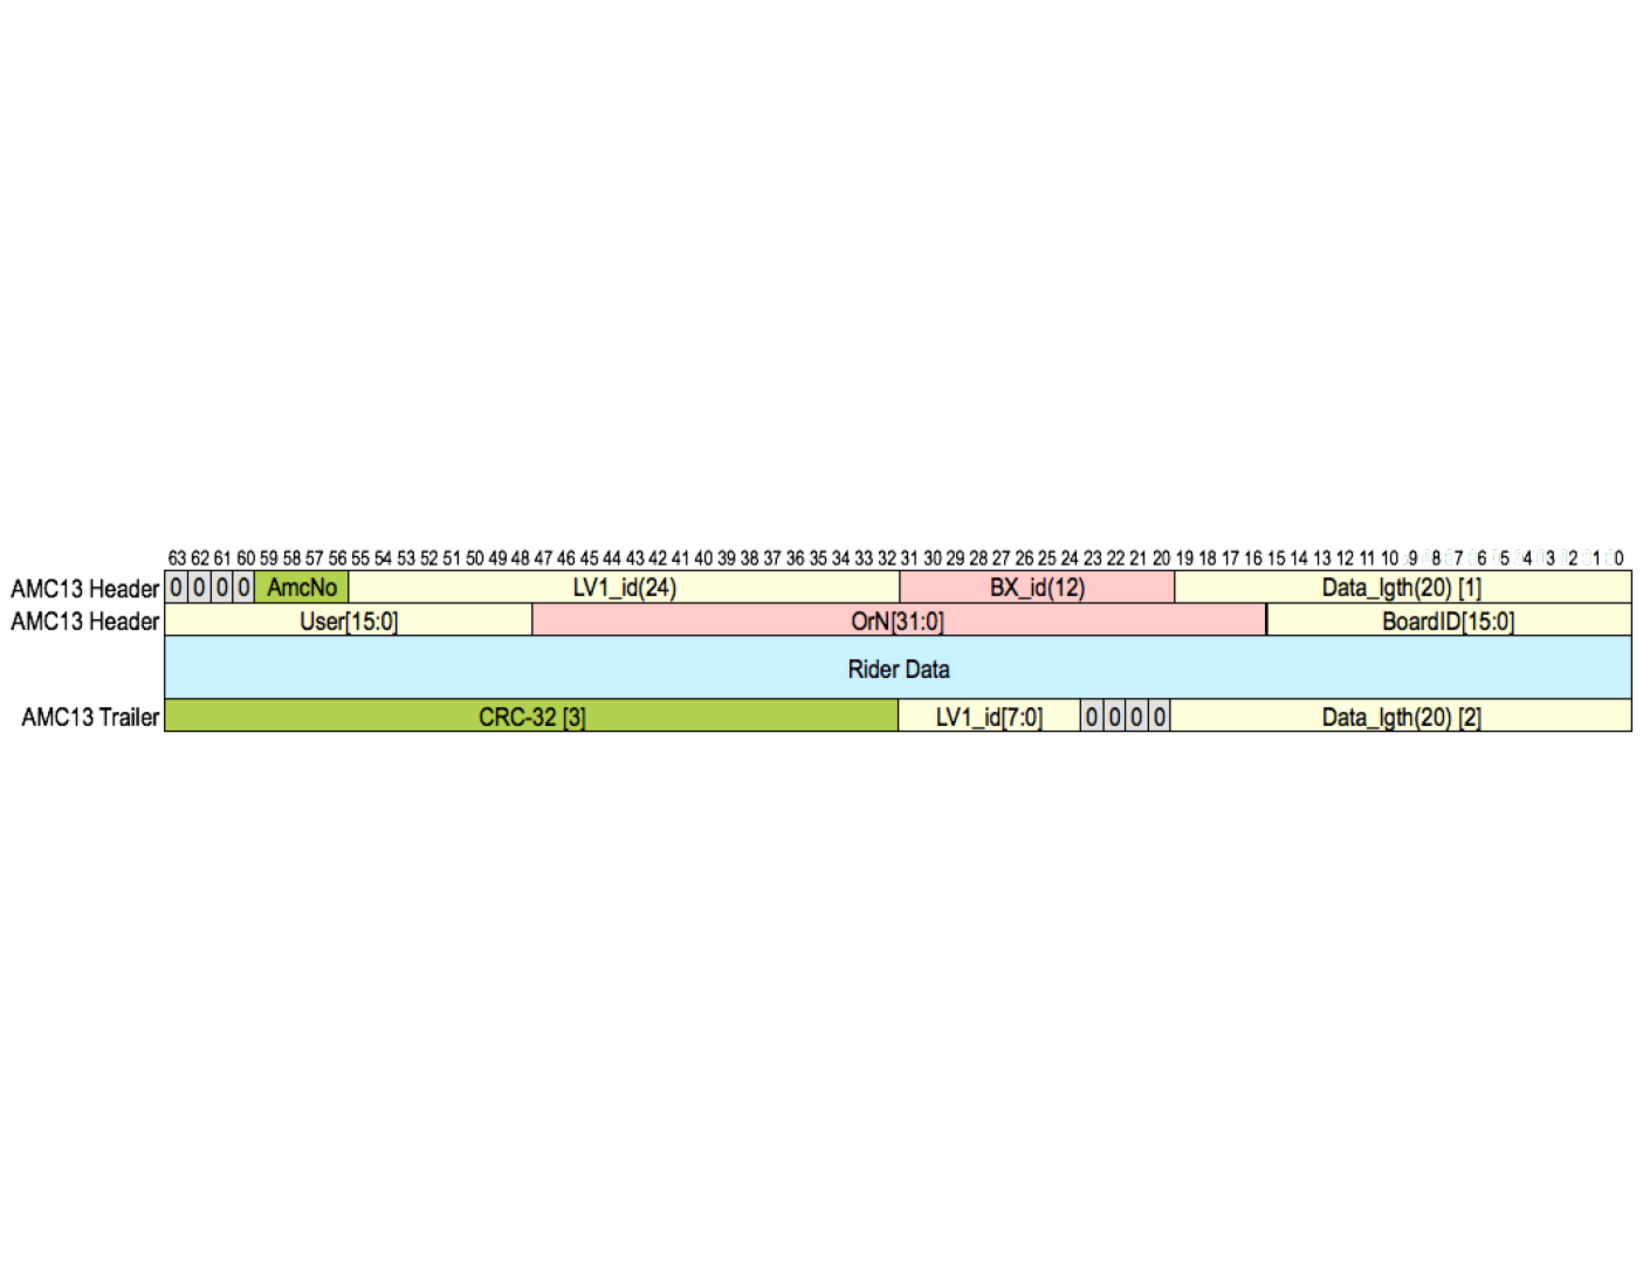
\includegraphics[trim=0cm 9.5cm 0cm 9.5cm ,width=0.95\textwidth]{pics/RiderToAMC13Header}
\caption{Rider to AMC13 data format.}
\end{figure}

%trim left bottom right top
\begin{figure}[htbp]
\centering
%\fbox{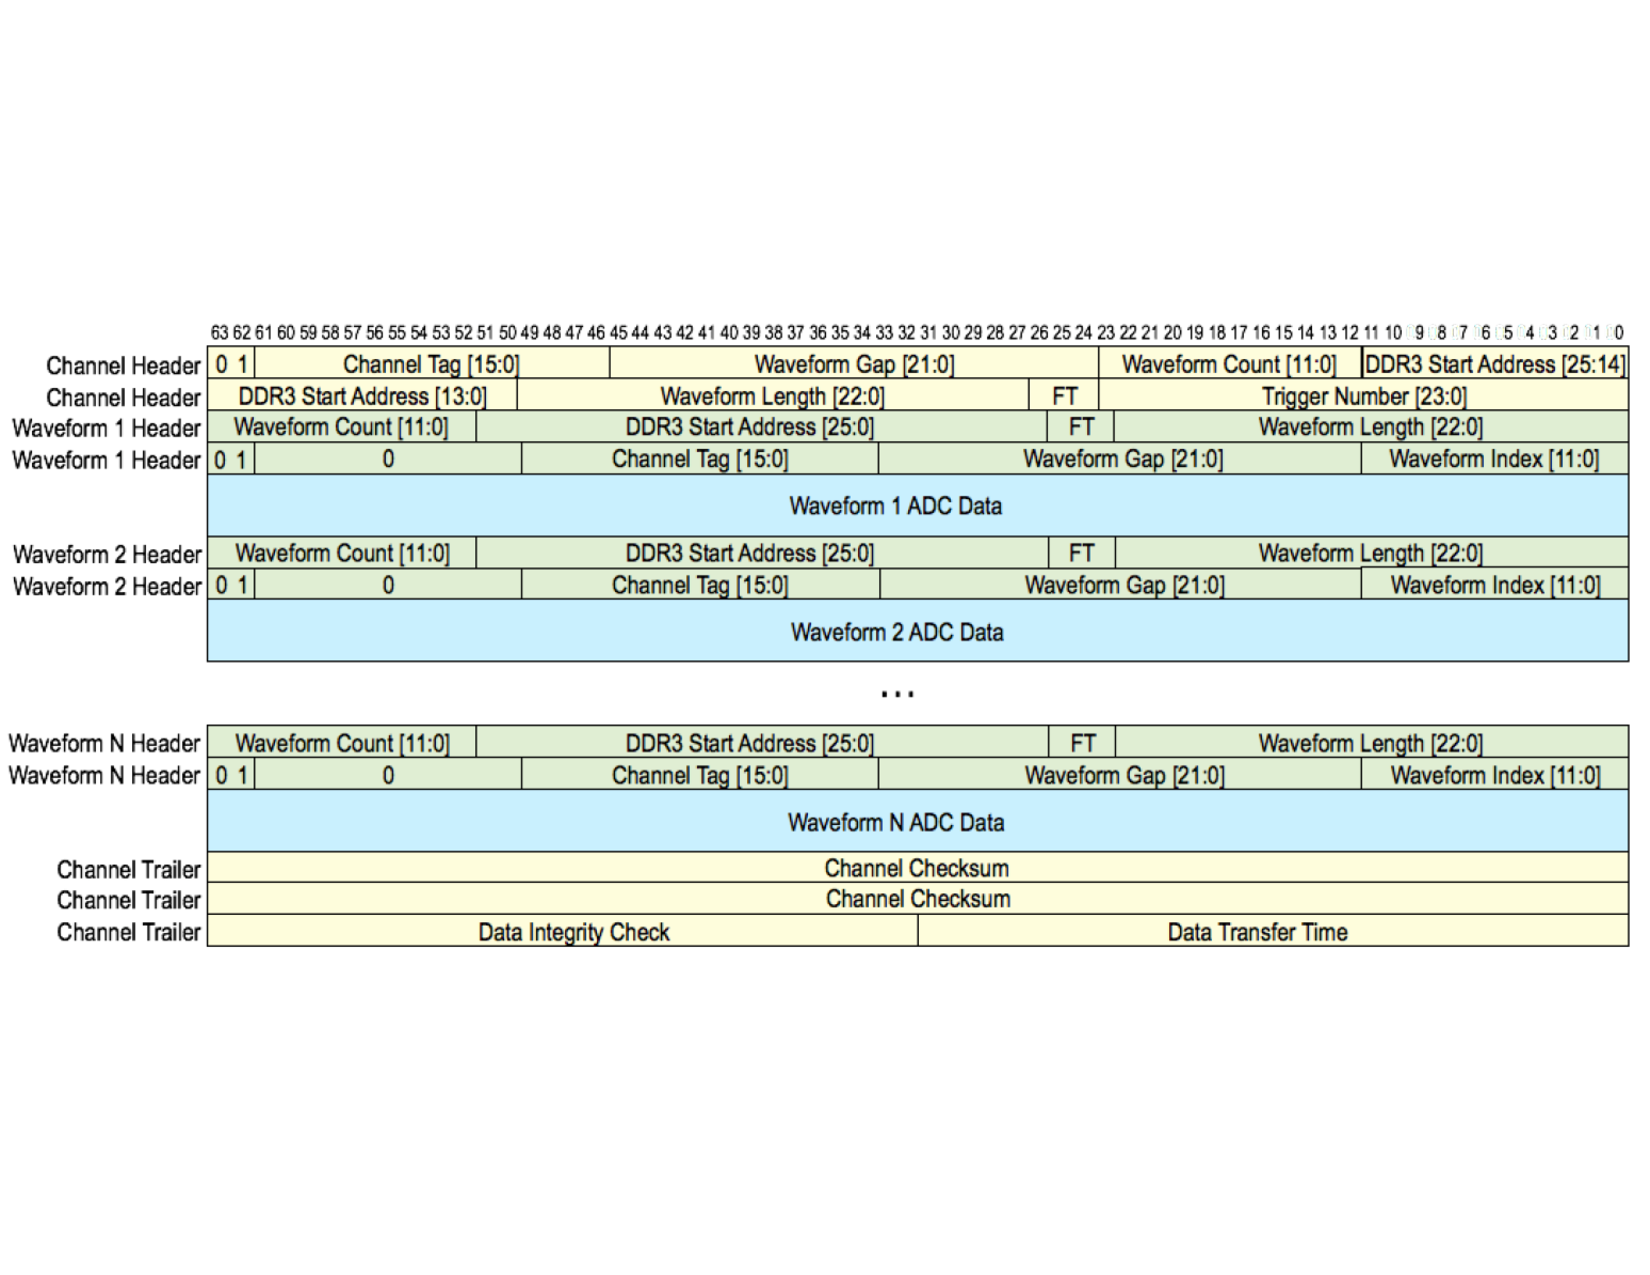
\includegraphics[trim=0cm 5.5cm 0cm 5.5cm ,width=0.9\textwidth]{pics/RiderChannelHeader}} guide line for trimming
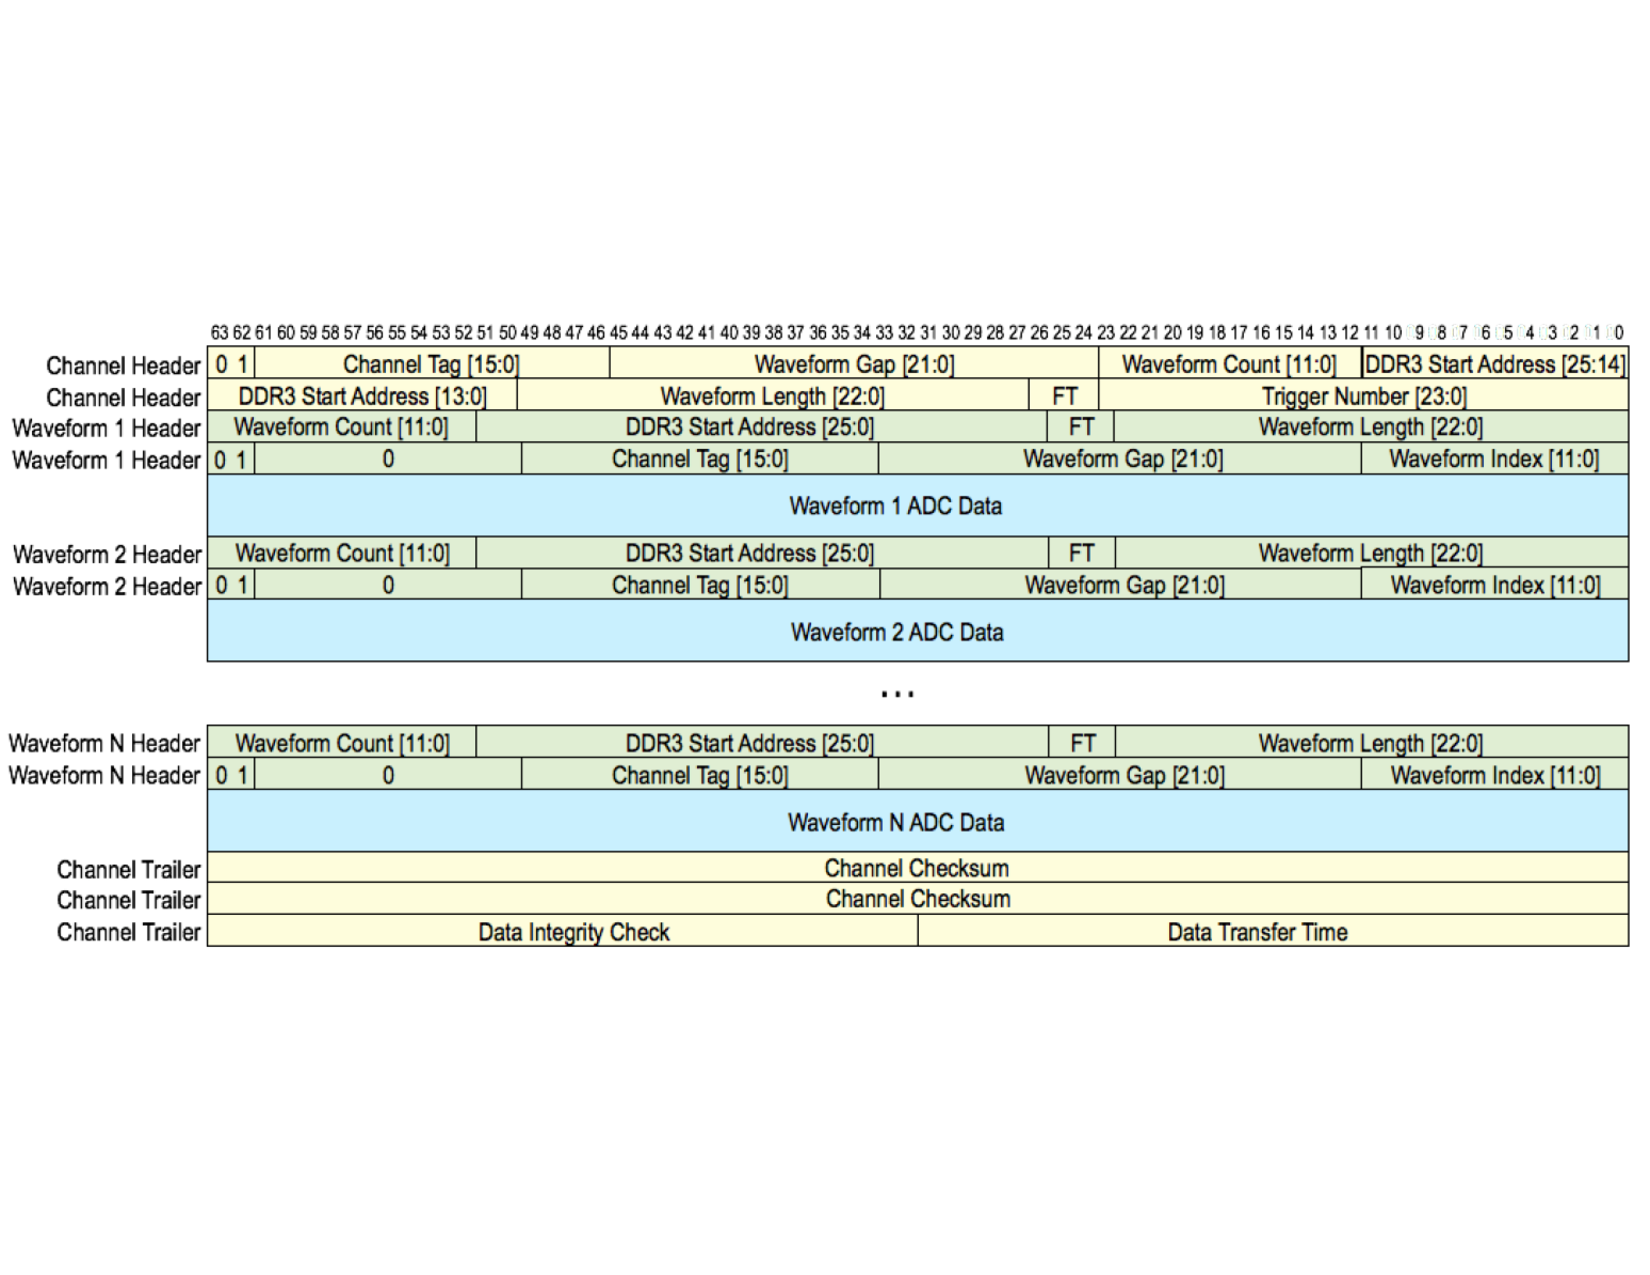
\includegraphics[trim=0cm 5.5cm 0cm 5.5cm ,width=0.95\textwidth]{pics/RiderChannelHeader}
\caption{Rider Channel data format.}
\end{figure}

\begin{figure}[htbp]
\centering
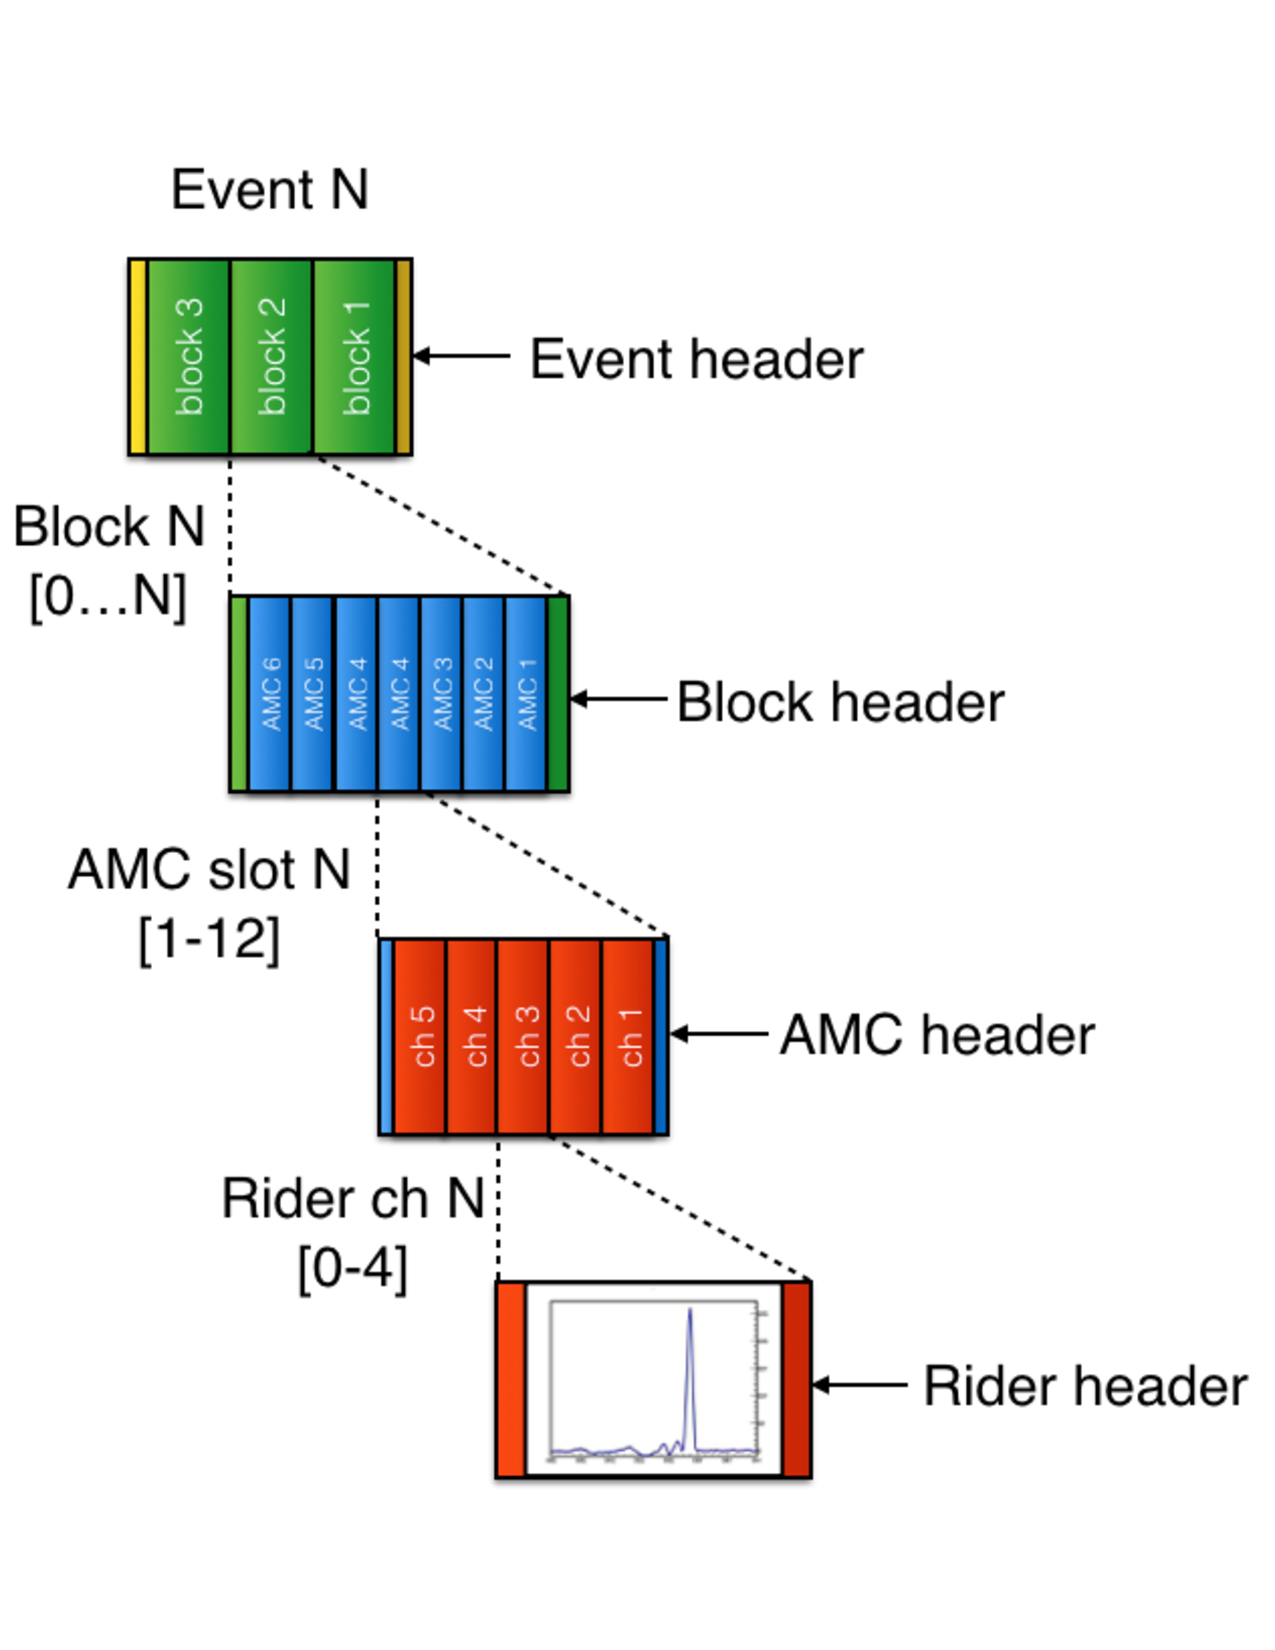
\includegraphics[width=0.9\textwidth]{pics/AllHeaders}
\caption{Per event data format}
\end{figure}

\section{Slow control data}

The only slow control data recorded by the MIDAS DAQ is the temperature sensor SCS-3000. It was initially installed in the control room and was moved into the experimental hall on Jun 8 2016 in the night. It has 6 channels and the corresponding locations are summarized in~\tref{tab:temp}.

\begin{table}[htbp]
\caption{Locations of the temperature sensors of SCS-3000.}
\begin{longtable}{|c|c|} \hline
ID &  Location \\ \hline
1 & Air in \\ \hline
2 & Loose on table in front of calorimeter \\ \hline
3 & Loose on table in front of calorimeter \\ \hline
4 & Loose on table in front of calorimeter \\ \hline
5 & Air out \\ \hline
6 & Tunnel entrance \\ \hline
\end{longtable}
\label{tab:temp}
\end{table}
